\documentclass[../main.tex]{subfiles}
\graphicspath{{\subfix{../images/}}}
\usepackage{subfiles}
\usepackage{subfig}

\begin{document}
    \subsection{Time Series}

    In this section, the properties inherent in time series analysis will be explored, as understanding their properties is essential for effective analysis and modeling. We will delve into the fundamental characteristics that define time series, such as stationarity, seasonality, trend, and autocorrelation. These properties provide valuable insights into the underlying patterns, trends, and dependencies within the data. By grasping these key concepts, we can develop robust methodologies for forecasting, anomaly detection, and decision-making based on time series data.

    \subsubsection{Properties}

        Now that we have established the significance of understanding and analyzing time series, let's delve deeper into the characteristics and properties of these series. To begin with, time series can be categorized as either \textbf{continuous} or \textbf{discrete}, depending on whether the observations are recorded continuously over time or at discrete intervals. For the purposes of our discussion, all the time series considered will be discrete in nature, even if the underlying variable being measured is continuous.\par

        Another crucial differentiation lies in the classification of time series as either \textbf{deterministic} or \textbf{stochastic} processes. A deterministic time series implies that its future values can be precisely predicted based on its past values, indicating a predictable pattern. On the other hand, a stochastic time series suggests that future values are not solely determined by past observations, rendering exact predictions unattainable. Instead, stochastic time series necessitate the concept of probability distribution to capture the uncertainty associated with future values. Again, all the time series that will be worked with will be stochastic in nature.\par

        One of the main ways of describing a stochastic process is through its moments, in particular the first (called the \textit{mean}, $\mu$) and second (called the autocovariance function, acv.f.) one, that can be defined as:

            $$\mu(t) = E[X(t)]$$
            $$acv.f. = \gamma (t_1,t_2) = E\{[X(t_1)-\mu(t_1)][X(t_2)-\mu(t_2)]\}$$

        with this, we can also define the autocorrelation ($\rho(\tau)$) as the normalized acv.f., .

            $$\rho(\tau) + \frac{\gamma(\tau)}{\gamma (0)}$$

        Another property of the time series that will be introduced here is \textbf{stationarity}. Simply put, a series is stationary if there is no systematic change in the mean value and variance and if purely cyclic variations have been removed. Mathematically, a time series is said to be strictly stationary if the joint distribution of X($t_1$), ..., X($t_k$) is the same as the one of X($t_1+\tau$), ..., X($t_k+\tau$) for any k. Because this is such a restrictive definition, in many instances it is better to use the looser \textbf{second-order stationarity}, that only requires that the mean is constant and that the autocovariance function only depends on the lag. One way to remove a trend in order to make the series more stationary is by differencing it (usually first order differencing is already enough).

        When dealing with a series that has a trend and a seasonal component, it is possible to analyze it by decomposing it in a trend, a periodic and a noise component. An example of such decomposition can be viewed in Figure \ref{fig:decomposition}. \par

        \begin{figure}[h]
            \begin{center}
            \centering
            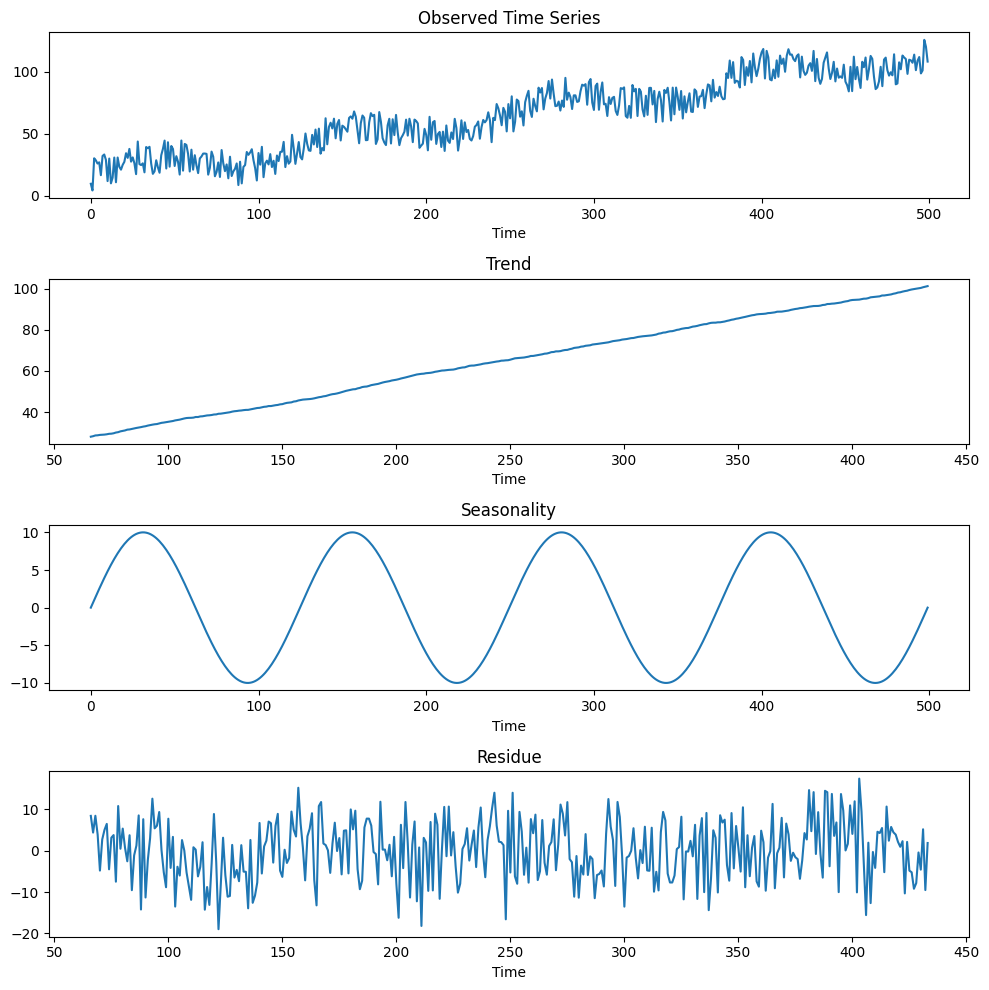
\includegraphics[width={0.8\columnwidth}]{images/trend_seas_res.png}
            \caption{Example of the decomposition of a signal in trend, seasonality and residual noise.}
            \label{fig:decomposition}
            \end{center}
        \end{figure}

        By considering these distinctions, we can gain a more comprehensive understanding of the various types of time series and their inherent properties. The goal of this work is around the description, explanation, prediction and simulation of time series.\par

    \subsubsection{Linear Time Series Models}
        In time series analysis, various models are used to describe the behavior and dynamics of the data. A purely random process is characterized by a sequence of random variables, denoted as {$Z_t$}, that are mutually independent and identically distributed (i.i.d.). Building upon this notion, we can define a random walk process, denoted as {$X_t$}, where each value is obtained by adding the current random variable, $Z_t$, to the previous value, $X_{t-1}$.

        $$X_t = X_{t-1} + Z_t$$

        Taking a step further, a moving average process of order $q$, denoted as MA($q$), can be formulated. In this model, the value of $X_t$ is determined by a linear combination of the most recent $q$ random variables, $Z_t$, $Z_{t-1}$, ..., $Z_{t-q}$, with respective coefficients $\beta_0$, $\beta_1$, ..., $\beta_q$.

        $$X_t = \beta_0Z_t + \beta_1Z_{t-1} + ...+ \beta_qZ_{t-q}$$

        Similarly, an autoregressive process of order $p$, denoted as AR($p$), is defined. In this case, the value of $X_t$ depends on a linear combination of the past $p$ values, $X_{t-1}$, $X_{t-2}$, ..., $X_{t-p}$, with respective coefficients $\alpha_0$, $\alpha_1$, ..., $\alpha_p$, along with the current random variable $Z_t$.

        $$X_t = \alpha_0X_{t-1} + \alpha_1X_{t-2} + ...+ \alpha_pX_{t-p} + Z_t$$
        
        It is worth noting that AR and MA processes are mathematically equivalent, and they can be combined to create other useful models. For instance, the combination of autoregressive and moving average components gives rise to the autoregressive moving average (ARMA) model. The inclusion of differencing, which involves computing the differences between consecutive observations, allows the use of ARMA models on non-stationary data, leading to the autoregressive integrated moving average (ARIMA) model. Additionally, the ARFIMA model incorporates long-range dependence by including fractional differencing in the time series analysis. \par

        By employing these various models, time series analysts can capture different patterns, trends, and dependencies present in the data, enabling a deeper understanding and facilitating effective forecasting and analysis.
    
    \subsubsection{Frequency Domain Analysis}
        Up until this point we discussed about analysing our time series in the time domain, meaning each sample corresponds to a point in time. Another complementary way of analysing our series would be by converting it to some other domain, such as the Frequency domain. This conversion can be done in many ways, such as the Fourier Transform or Wavelet Transforms.   

\end{document}